\documentclass[a4paper,titlepage,11pt,floatssmall]{mwrep}
\usepackage[left=2.5cm,right=2.5cm,top=2.5cm,bottom=2.5cm]{geometry}
\usepackage[OT1]{fontenc}
\usepackage{polski}
\usepackage{amsmath}
\usepackage{amsfonts}
\usepackage{amssymb}
\usepackage{graphicx}
\usepackage{float}
\usepackage{subfig}
\usepackage{url}
\usepackage{tikz}
\usetikzlibrary{arrows,calc,decorations.markings,math,arrows.meta}
\usepackage{rotating}
\usepackage[percent]{overpic}
\usepackage[utf8]{inputenc}
\usepackage{xcolor}
\usepackage{colortbl}
\usepackage{listings}
\usepackage{matlab-prettifier}
\usepackage{enumitem,amssymb}
\definecolor{szary}{rgb}{0.95,0.95,0.95}
\usepackage{siunitx}
\sisetup{detect-weight,exponent-product=\cdot,output-decimal-marker={,},per-mode=symbol,range-phrase={-},range-units=single}

%konfiguracje pakietu listings
\lstset{
  literate={ą}{{\k a}}1
           {Ą}{{\k A}}1
           {ż}{{\. z}}1
           {Ż}{{\. Z}}1
           {ź}{{\' z}}1
           {Ź}{{\' Z}}1
           {ć}{{\' c}}1
           {Ć}{{\' C}}1
           {ę}{{\k e}}1
           {Ę}{{\k E}}1
           {ó}{{\' o}}1
           {Ó}{{\' O}}1
           {ń}{{\' n}}1
           {Ń}{{\' N}}1
           {ś}{{\' s}}1
           {Ś}{{\' S}}1
           {ł}{{\l}}1
           {Ł}{{\L}}1
}
\lstset{
	backgroundcolor=\color{szary},
	frame=single,
	breaklines=true,
}
\lstdefinestyle{customlatex}{
	basicstyle=\footnotesize\ttfamily,
	%basicstyle=\small\ttfamily,
}
\lstdefinestyle{customc}{
	breaklines=true,
	frame=tb,
	language=C,
	xleftmargin=0pt,
	showstringspaces=false,
	basicstyle=\small\ttfamily,
	keywordstyle=\bfseries\color{green!40!black},
	commentstyle=\itshape\color{purple!40!black},
	identifierstyle=\color{blue},
	stringstyle=\color{orange},
}
\lstdefinestyle{custommatlab}{
	captionpos=t,
	breaklines=true,
	frame=tb,
	xleftmargin=0pt,
	language=matlab,
	showstringspaces=false,
	basicstyle=\small\ttfamily,
	%basicstyle=\scriptsize\ttfamily,
	keywordstyle=\bfseries\color{green!40!black},
	commentstyle=\itshape\color{purple!40!black},
	identifierstyle=\color{blue},
	stringstyle=\color{orange},
}
\lstdefinestyle{custompython}{
	captionpos=t,
	breaklines=true,
	frame=tb,
	xleftmargin=0pt,
	language=python,
	showstringspaces=false,
	basicstyle=\small\ttfamily,	
	keywordstyle=\bfseries\color{green!40!black},
	commentstyle=\itshape\color{purple!40!black},
	identifierstyle=\color{blue},
	stringstyle=\color{orange},
}

%wymiar tekstu (bez żywej paginy)
\textwidth 160mm \textheight 247mm

\def\figurename{Rys.}
\def\tablename{Tab.}

%konfiguracja liczby pływających elementów
\setcounter{topnumber}{0}%2
\setcounter{bottomnumber}{3}%1
\setcounter{totalnumber}{5}%3
\renewcommand{\textfraction}{0.01}%0.2
\renewcommand{\topfraction}{0.95}%0.7
\renewcommand{\bottomfraction}{0.95}%0.3
\renewcommand{\floatpagefraction}{0.35}%0.5

\begin{document}
\frenchspacing
\pagestyle{uheadings}

%strona tytułowa
\title{\bf Zastosowanie modeli statyki typu Takagi-Sugeno z następnikami hiperbolicznymi w algorytmach regulacji predykcyjnej}
\author{Wojciech Rogalski}
\date{2024}

\makeatletter
\renewcommand{\maketitle}{\begin{titlepage}
\begin{center}{\LARGE {\bf
Wydział Elektroniki i Technik Informacyjnych}}\\
\vspace{0.4cm}
{\LARGE {\bf Politechnika Warszawska}}\\
\vspace{0.3cm}
\end{center}
\vspace{5cm}
\begin{center}
{\bf \LARGE Pracownia dyplomowa magisterska \vskip 0.1cm}
(semestr letni 23/24L)
\end{center}
\vspace{1cm}
\begin{center}
{\bf \LARGE \@title \vskip 0.1cm}
\end{center}
\vspace{2cm}
\begin{center}
\begin{tabular}{@{}c@{\hspace{2cm}}c@{}}
\bf \Large Autor: & \bf \Large Promotor: \\
\@author & dr hab. inż. Piotr Marusak
\end{tabular}
\end{center}
\vspace*{\stretch{6}}
\begin{center}
\bf{\large{Warszawa, \@date\vskip 0.1cm}}
\end{center}
\end{titlepage}
}
\makeatother
\maketitle
\tableofcontents

\chapter{Wstęp}
Praca zawiera porównanie modeli Hammersteina oraz Wienera w regulacji kaskadowej. Bazą porównania był obiekt opisany równaniami fizycznymi postaci:
\begin{equation}
\begin{cases}
\frac{dV_1}{dt} = F_1 + F_D - F_2(h_1) \\
\frac{dV_2}{dt} = F_2(h_1) - F_3(h_2) \\
F_2(h_1) = \alpha_1 \sqrt{h_1}, \quad F_3(h_2) = \alpha_2 \sqrt{h_2}, \quad V_1(h_1) = A_1h_1, \quad V_2(h_2) = C_2h_2^2, \quad F_1(t) = F_{1in}(t-\tau)  
\end{cases}
\label{model_fiz}
\end{equation}

\begin{itemize}
\item[•] Stałe: 
\begin{equation}
A_1 = 540cm^2, \quad C_2 = \num{0.85}, \quad \alpha_1 = 26, \quad \alpha_2 = 20
\end{equation}

\item[•] Punkt pracy:
\begin{equation}
F_1 = 90 \frac{cm^3}{s}, \quad F_D = 30 \frac{cm^3}{s}, \quad \tau = 100, \quad h_2 = 36cm
\end{equation}
\end{itemize}

\noindent gdzie użyte oznaczenia odpowiadają tym zastosowanym na rys. \ref{schemat}.

\begin{figure}[h!]
\centering
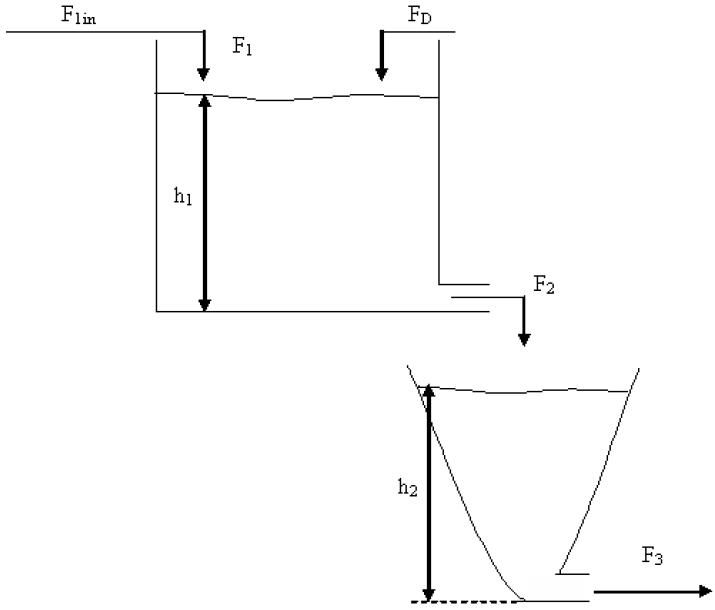
\includegraphics[width=0.8\textwidth]{pictures/schemat}
\caption{Obiekt regulacji automatycznej.}
\label{schemat}
\end{figure}

Wartością sterującą był dopływ $F_{1in}$ natomiast zakłóceniem - $F_D$. Z kolei wyjściem - wartością regulowaną - wysokość cieczy w drugim zbiorniku $h_2$. W pierwszej kolejności dokonano identyfikacji modelu, sprawdzono jego nieliniowość i dobrano odpowiedni rząd dynamiki modelu liniowego.
\chapter{Identyfikacja}
\section{Charakterystyka statyczna}
Poświęcono jej bardzo dużo uwagi, ze względu na kluczową rolę, jaką odgrywa we wspomnianych modelach Hammersteina i Wienera. Korzystając z modelu fizycznego, z równania \ref{model_fiz} wyznaczono:
\begin{equation}
\frac{dV_1}{dt} = 0 \quad \wedge \quad \frac{dV_2}{dt} = 0
\end{equation}

\noindent wobec tego:
\begin{equation}
\begin{cases}
F_1 + F_D - \alpha_1 \sqrt{h_1} &= 0 \\
\alpha_1 \sqrt{h_1} - \alpha_2 \sqrt{h_2} &= 0
\end{cases}
\end{equation}

\noindent Po prostych przekształceniach otrzymano wzór opisujący charakterystykę statyczną:
\begin{equation}
h_2 = \left( \frac{F_1 + F_D}{\alpha_2} \right)^2
\end{equation}

\noindent Wykres odpowiadający wyprowadzonemu wzorowi prezentuje się następująco:

\begin{figure}[h!]
\centering
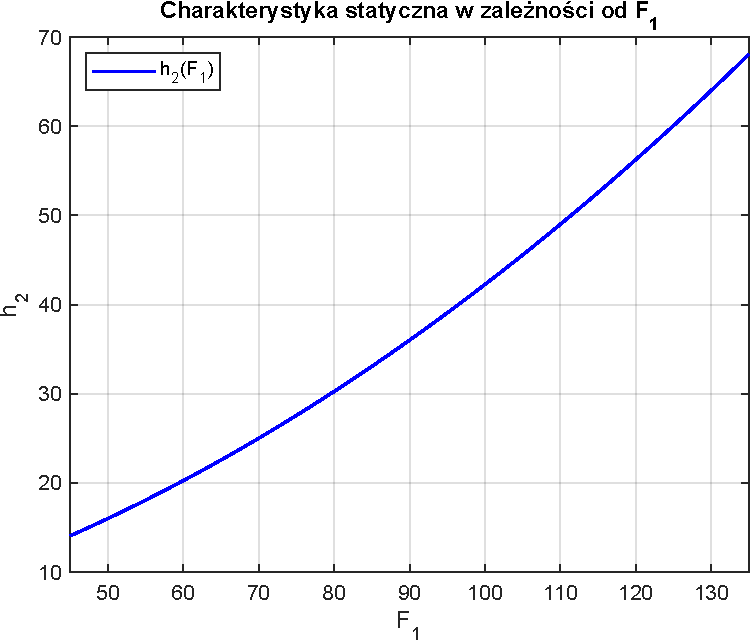
\includegraphics[width=0.8\textwidth]{pictures/static_characteristic}
\caption{Charakterystyka statyczna $h_2(F_1)$.}
\label{static_characteristic}
\end{figure}

\noindent Założono przedział zmienności sygnału sterującego w zakresie $F_1 \in [-45, 45]$.

\newpage

\section{Wymuszenia}
Po dokonaniu pierwszego kroku identyfikacji - wykreślenia charakterystyki statycznej - uzyskano wstępne informacje o obiekcie. Równania opisujące model (\ref{model_fiz}) oraz charakterystyka statyczna przedstawiona na rys. \ref{static_characteristic} pokazuje, że obiekt jest nieliniowy, stąd dokonano jego linearyzacji w punkcie pracy, tj.:
\begin{equation}
\begin{cases}
\frac{dV_1}{dt} \cong F_1 + F_D - \alpha_1 \sqrt{\frac{V_{10}}{A}} - \frac{\alpha_1}{2 \sqrt{A \cdot V_{10}}} \cdot (V_1 - V_{10})\\
\frac{dV_2}{dt} \cong \alpha_1 \sqrt{\frac{V_{10}}{A}} - \alpha_2 \sqrt[4]{\frac{V_{20}}{C}} + \frac{\alpha_1}{2 \sqrt{A \cdot V_{10}}} \cdot (V_1 - V_{10}) - \frac{\alpha_2}{4 \sqrt[4]{C \cdot V_{20}^3}} \cdot (V_2 - V_{20})
\end{cases}
\end{equation}

\noindent Linearyzacji dokonano przyjmując jako zmienną stanu objętość cieczy w obu zbiornikach. 

\begin{equation}
x = \begin{bmatrix} V_1 & V_2 \end{bmatrix}^T
\end{equation}

Następnie, podając wygenerowaną sekwencję sygnału sterującego, zbadano rozbieżność modelu liniowego i nieliniowego.

\begin{figure}[h!]
\centering
\subfloat[Wygenerowana sekwencja sygnału sterującego $u(k)$.]{
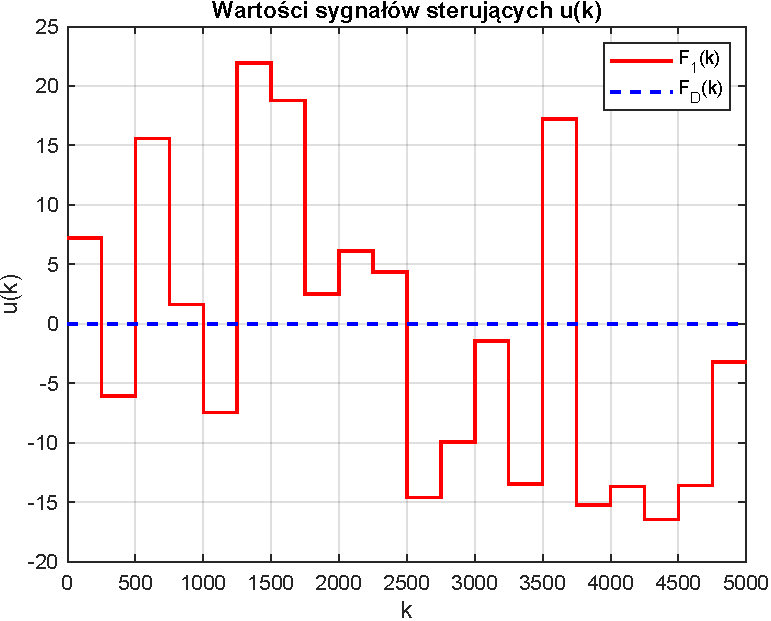
\includegraphics[width=0.45\textwidth]{pictures/u_F1}}
\hfill
\subfloat[Sygnał wyjściowy $y(k)$.]{
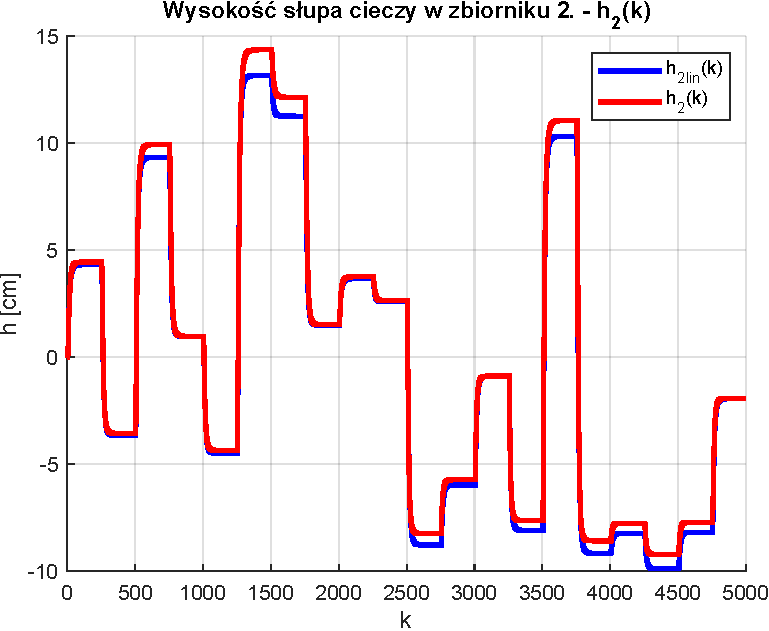
\includegraphics[width=0.45\textwidth]{pictures/y_F1}}
\caption{Porównanie modelu liniowego z nieliniowym.}
\end{figure}

Otrzymano dokładnie to czego się spodziewano. Wymuszenia nie większe niż $\pm 10 \frac{cm^3}{s}$ nie powodują znacznego wytrącenia układu z położenia równowagi, dzięki czemu model liniowy bardzo dobrze aproksymuje zachowanie układu. Niestety sytuacja pogarsza się wraz z oddalaniem się od punktu pracy - model liniowy zaczyna poważnie odbiegać od modelu nieliniowego, opisującego obiekt. W celach porównawczych policzono błędy, testując model w trybie bez rekurencji (ARX) oraz z rekurencją OE, przyjmując jako kryterium jakości błąd średni kwadratowy, tj.:

\begin{equation}
E = \sum_{k=0}^N (y(k) - y^{mod}(k))^2
\end{equation}

\noindent Wcześniej dokonano podziału wygenerowanych danych dynamicznych na dwa zbiory - uczący i~weryfikujący - stosując zasadę podziału $0\% - 50\% / 50\% - 100\%$, potrzebne do późniejszego, ewentualnego dostrajania modelu. Otrzymano następujące wyniki:

\begin{description}
\item[ARX] 
\begin{equation}
E_{ucz} = \num{0.002} \hspace{1cm} E_{wer}=\num{0.003}
\end{equation}
\item[OE] 
\begin{equation}
E_{ucz} = \num{0.470} \hspace{1cm} E_{wer}=\num{0.831}
\end{equation}
\end{description}

%\newpage

\begin{figure}[p!]
\begin{center}
\Large \textbf{Model ARX}
\end{center} 
\centering
\subfloat[Zbiór uczący.]{
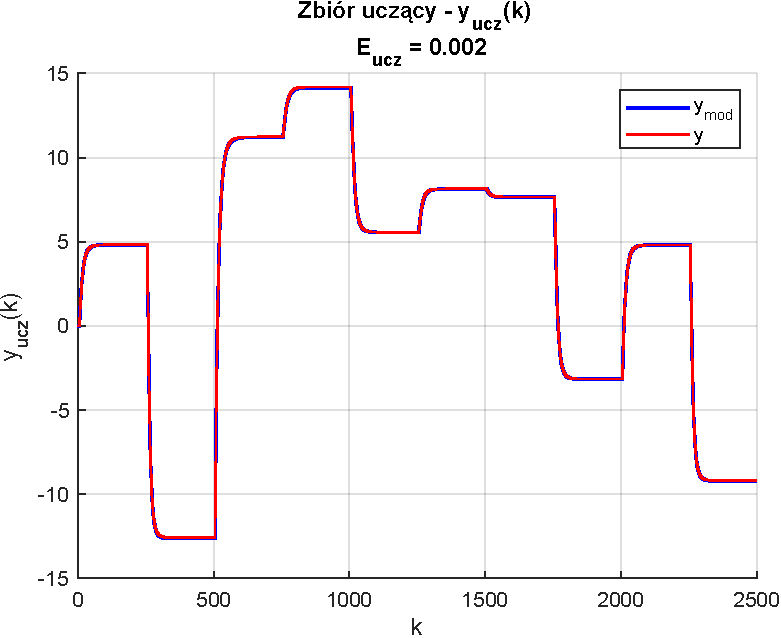
\includegraphics[width=0.45\textwidth]{pictures/arx_ucz}}
\hfill
\subfloat[Zbiór weryfikujący.]{
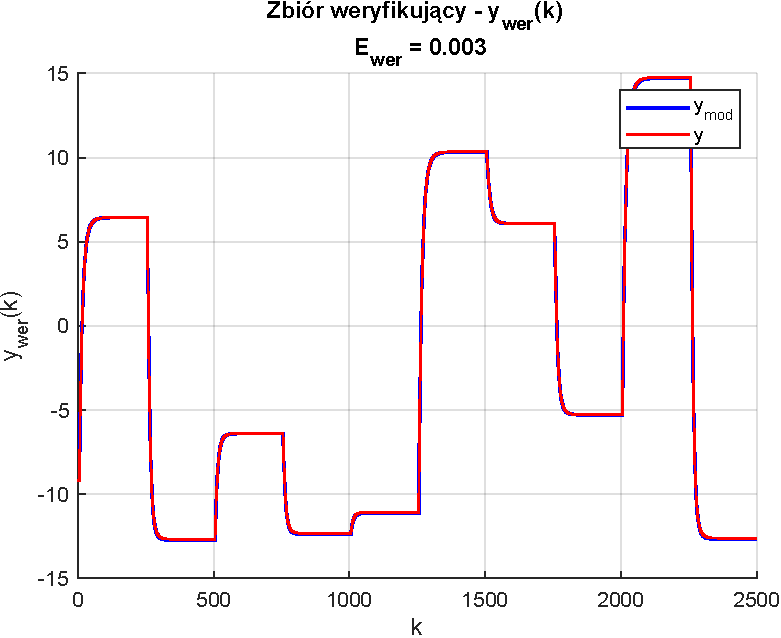
\includegraphics[width=0.45\textwidth]{pictures/arx_wer}}

\begin{center}
\Large \textbf{Model OE}
\end{center} 
\subfloat[Zbiór uczący.]{
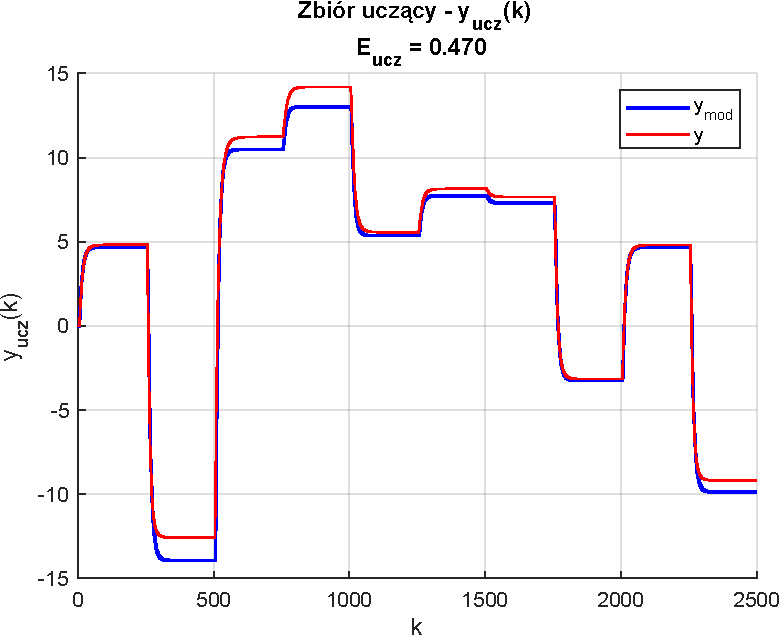
\includegraphics[width=0.45\textwidth]{pictures/oe_ucz}}
\hfill
\subfloat[Zbiór weryfikujący.]{
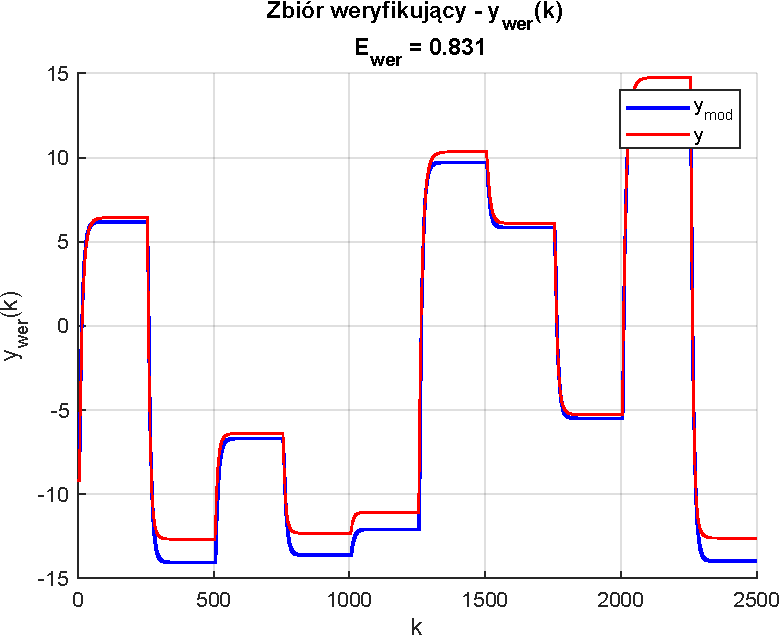
\includegraphics[width=0.45\textwidth]{pictures/oe_wer}}
\caption{Symulacja odpowiednich modeli z wykorzystaniem wygenerowanej sekwencji sygnału sterującego.}
\end{figure}

\newpage

\section{Podejście inżynierskie}
Od tej pory do dalszej analizy postanowiono przyjąć model szarej skrzynki. Informacją o obiekcie był fakt, że układ był inercyjny. Zadano więc wymuszenie w postaci skoku jednostkowego i starano się aproksymować odpowiedź układu dobierając odpowiednie parametru dla modelu transmitancji \textit{First Order Plus Dead Time} (FOPDT), który wyraża się wzorem:

\begin{equation}
G(s) = \frac{K_0e^{-sT_0}}{T_1s + 1}
\end{equation}

\noindent Dobrane parametry:

\begin{equation}
K_0 = \num{0.6025} \hspace{1cm} T_0 = 100 \hspace{1cm} T_1 = 225
\end{equation}

\begin{figure}[h!]
\centering
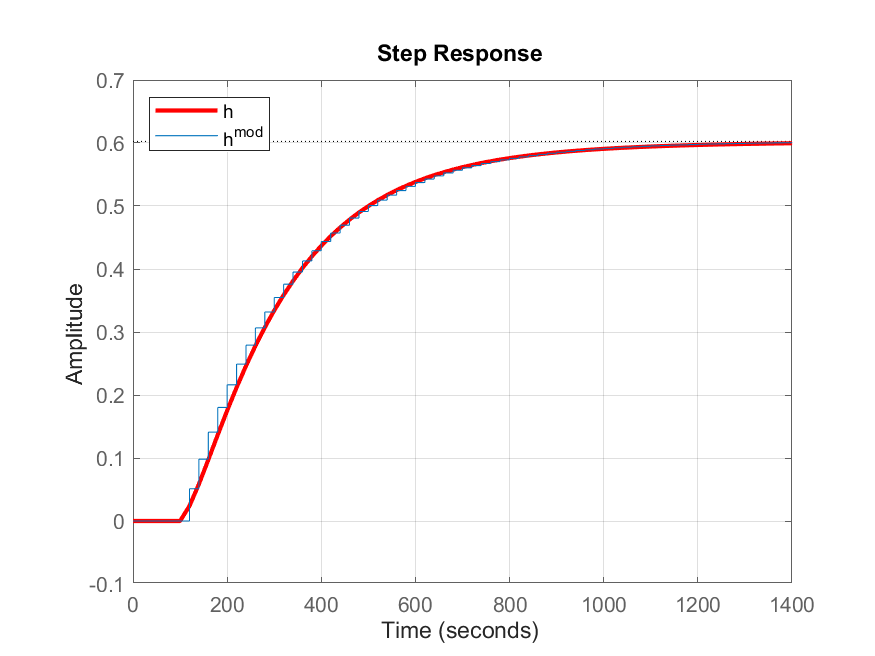
\includegraphics[width=\textwidth]{pictures/model_fopdt}
\caption{Aproksymacja odpowiedzi skokowej układu modelem FOPDT.}
\end{figure}

\newpage

Uzyskany rezultat nie był satysfakcjonujący stąd przyjęto model \textit{Second Order Plus Dead Time} (SOPDT), tj.

\begin{equation}
G(s) = \frac{K_0e^{-sT_0}}{(T_1s + 1)(T_2s + 1)}
\end{equation}

\noindent Dobrane parametry:

\begin{equation}
K_0 = \num{0.6025} \hspace{1cm} T_0 = 100 \hspace{1cm} T_1 = 212 \hspace{1cm} T_2 = 15
\end{equation}

\noindent Wynik prezentował się następująco:

\begin{figure}[h!]
\centering
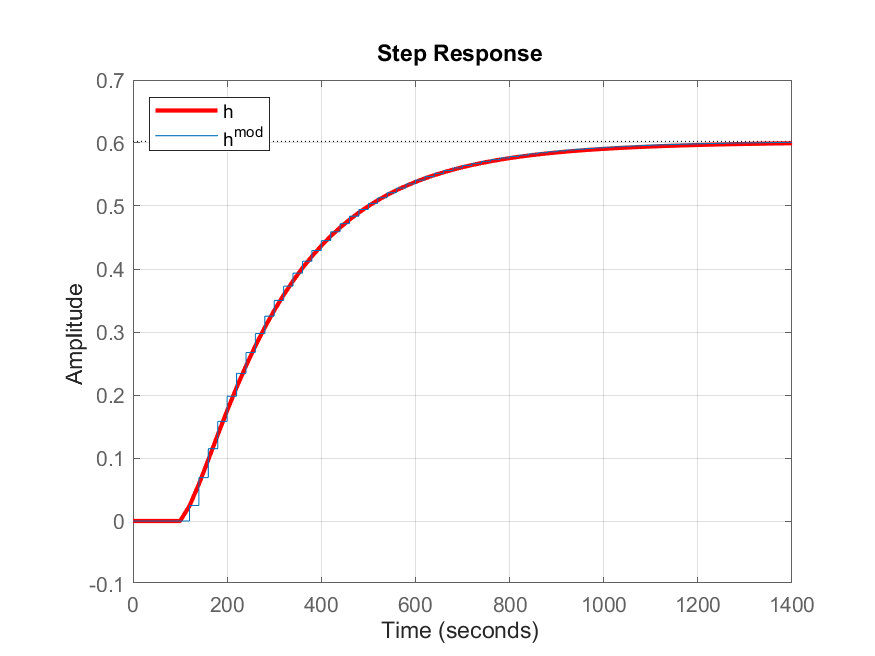
\includegraphics[width=\textwidth]{pictures/model_sopdt}
\caption{Aproksymacja odpowiedzi skokowej układu modelem SOPDT.}
\end{figure}

\newpage

Ponownie, chcąc sprawdzić skuteczność aproksymacji obiektu regulacji wygenerowanym modelem, którego równanie różnicowe jest postaci:

\begin{equation}
\begin{aligned}
y(k) = \num{1.174} y(k-1) - \num{0.2399} y(k-2) + &\num{0.02459} u_1(k-6) + \num{0.01536} u_1(k-7) \\ 
+&\num{0.02459} u_2(k-1) + \num{0.01536} u_2(k-2) 
\end{aligned}
\label{diff_eq}
\end{equation}

\noindent wygenerowano sekwencję sygnału sterującego $u_1(k)$ oraz $u_2(k)$, który są przyrostami wartości sterujących odpowiednio $F_1$ oraz $F_D$.

\begin{figure}[h!]
\begin{center}
\Large \textbf{Model ARX}
\end{center} 
\centering
\subfloat[Zbiór uczący.]{
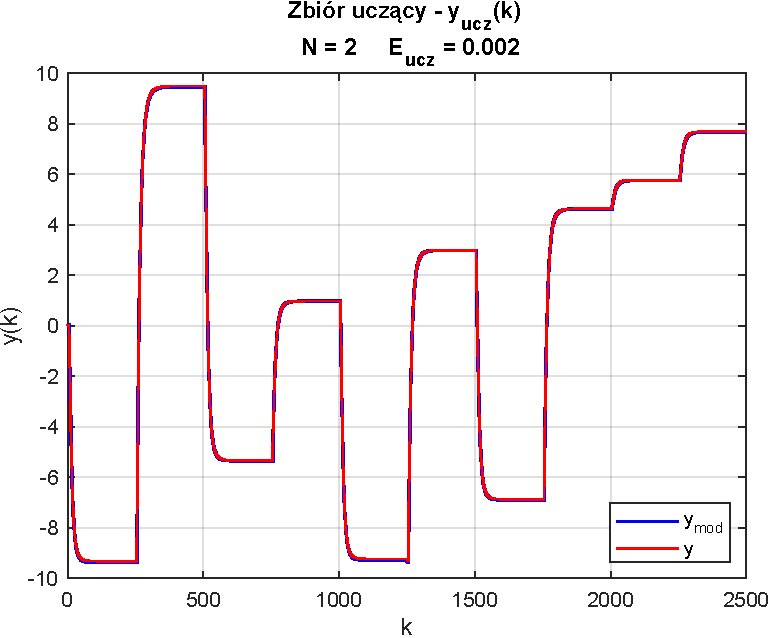
\includegraphics[width=0.45\textwidth]{pictures/arx_ucz_sopdt}}
\hfill
\subfloat[Zbiór weryfikujący.]{
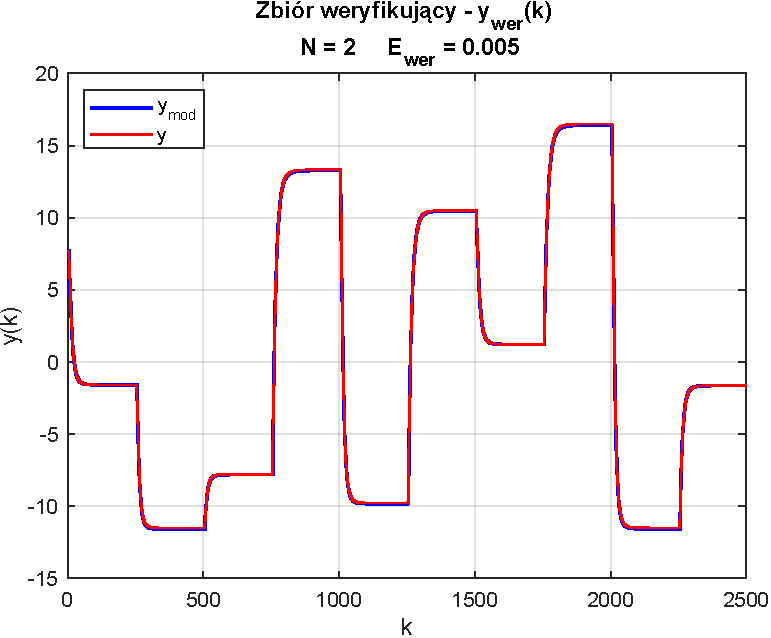
\includegraphics[width=0.45\textwidth]{pictures/arx_wer_sopdt}}

\begin{center}
\Large \textbf{Model OE}
\end{center} 
\subfloat[Zbiór uczący.]{
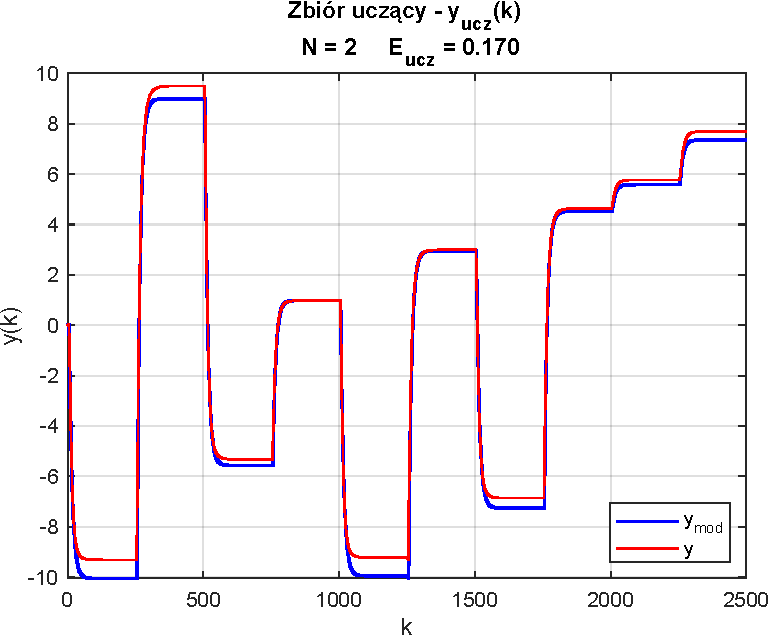
\includegraphics[width=0.45\textwidth]{pictures/oe_ucz_sopdt}}
\hfill
\subfloat[Zbiór weryfikujący.]{
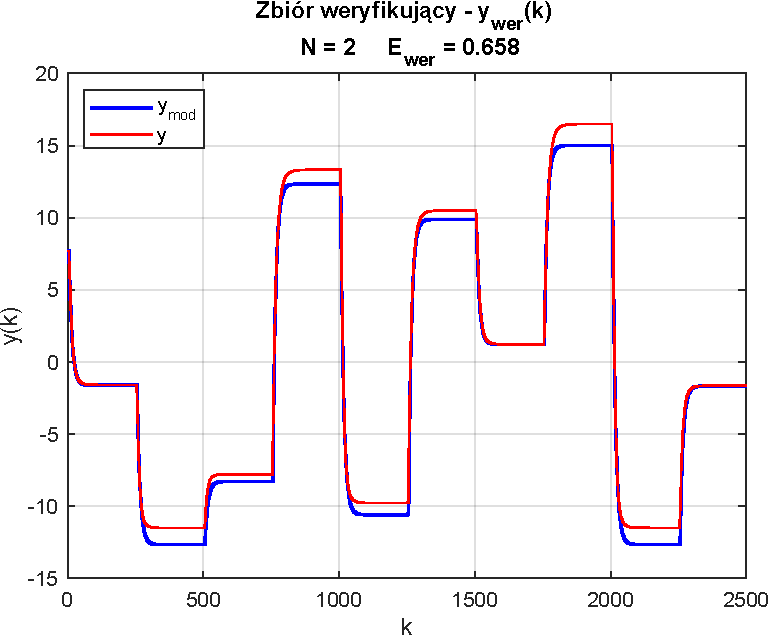
\includegraphics[width=0.45\textwidth]{pictures/oe_wer_sopdt}}
\caption{Symulacja odpowiednich modeli z wykorzystaniem wygenerowanej sekwencji sygnału sterującego.}
\end{figure}

Błędy uznano za akceptowalne na tym poziomie identyfikacji i przyjęto wyznaczony model do dalszej analizy.
\chapter{Porównanie}

\begin{figure}[h!]
\centering
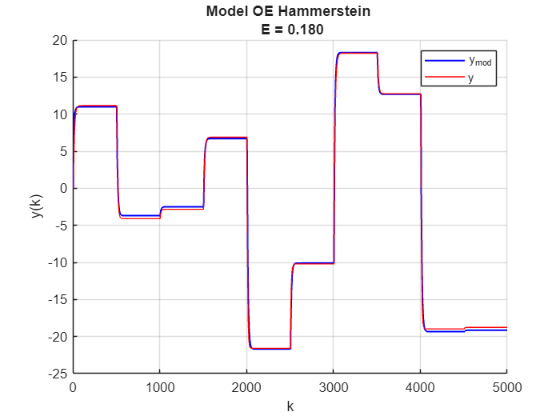
\includegraphics[width=0.7\textwidth]{pictures/model_hammersteina}
\caption{Model Hammersteina - następniki nieliniowe..}
\end{figure}

\begin{figure}[h!]
\centering
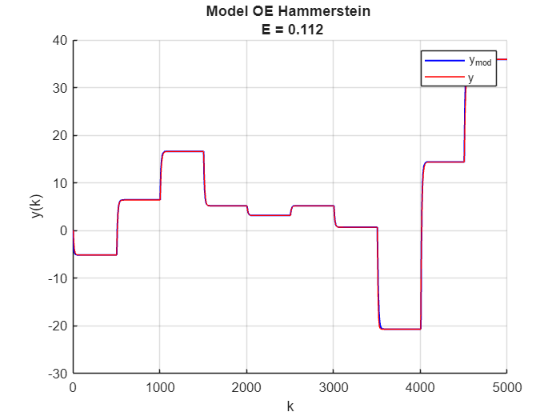
\includegraphics[width=0.7\textwidth]{pictures/model_hammersteina_lin}
\caption{Model Hammersteina - następniki liniowe.}
\end{figure}

\newpage

\begin{figure}[h!]
\centering
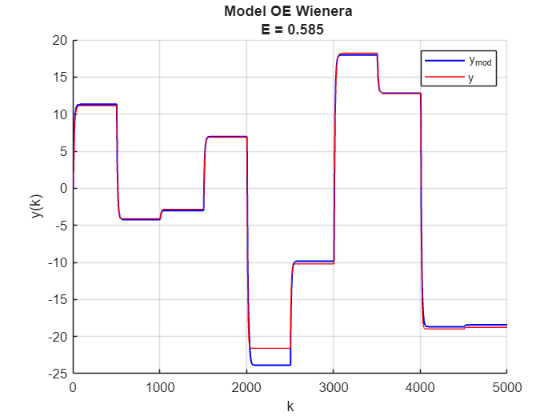
\includegraphics[width=0.7\textwidth]{pictures/model_wienera}
\caption{Model Wienera - następniki nieliniowe.}
\end{figure}

\begin{figure}[h!]
\centering
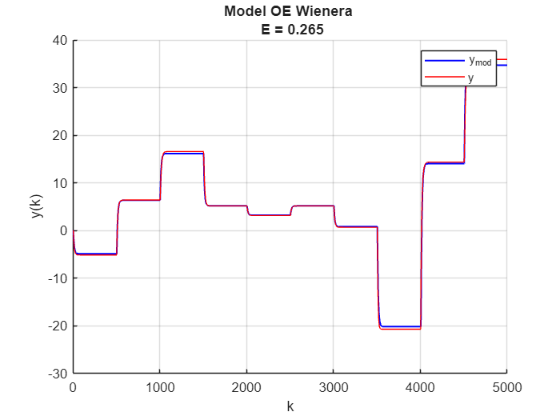
\includegraphics[width=0.7\textwidth]{pictures/model_wienera_lin}
\caption{Model Wienera - następniki liniowe.}
\end{figure}

\newpage

\begin{figure}[h!]
\centering
\includegraphics[width=\textwidth]{pictures/model_OE}
\caption{Model liniowy.}
\end{figure}

Zastosowania modeli zarówno Hammersteina, jak i Wienera przynosi duże korzyści w stosunku do samego modelu liniowego. Natomiast zastosowanie nieliniowych funkcji w następnikach reguł modelu Takagi-Sugeno pozwala zredukować liczbę zbiorów rozmytych nieznacznie tracąc na dokładności.
\chapter{DMC}

\begin{figure}[h!]
\centering
\subfloat{
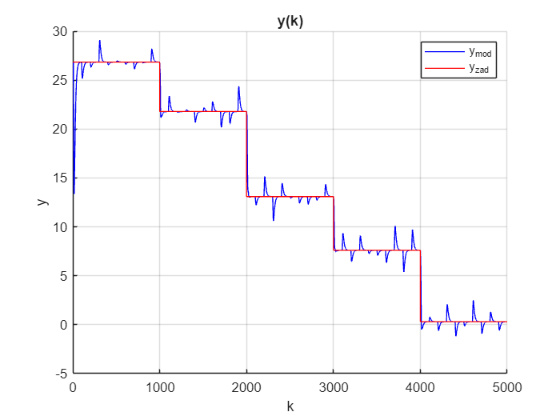
\includegraphics[width=0.8\textwidth]{pictures/dmc_analitic_y_z}}
\hfill
\subfloat{
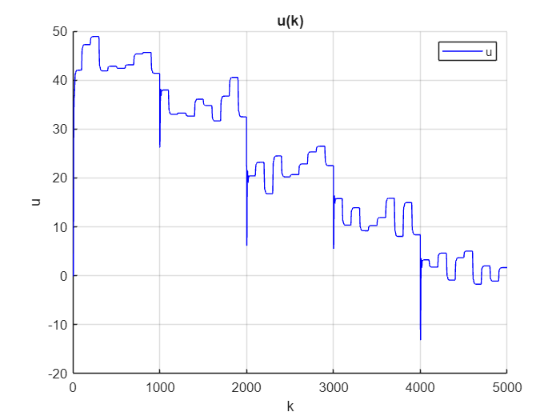
\includegraphics[width=0.8\textwidth]{pictures/dmc_analitic_u_z}}
\caption{Algorytm analityczny DMC bez pomiaru zakłóceń.}
\end{figure}

\newpage

\begin{figure}[h!]
\centering
\subfloat{
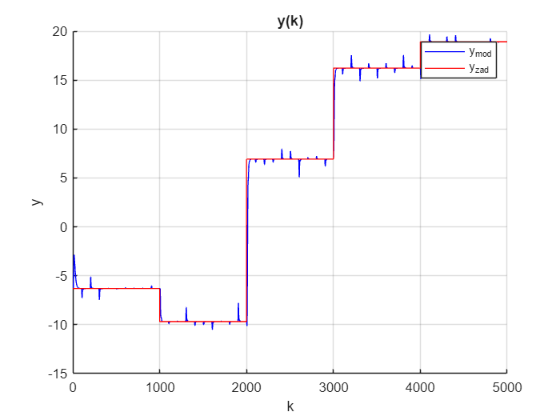
\includegraphics[width=0.8\textwidth]{pictures/dmc_analitic_y}}
\hfill
\subfloat{
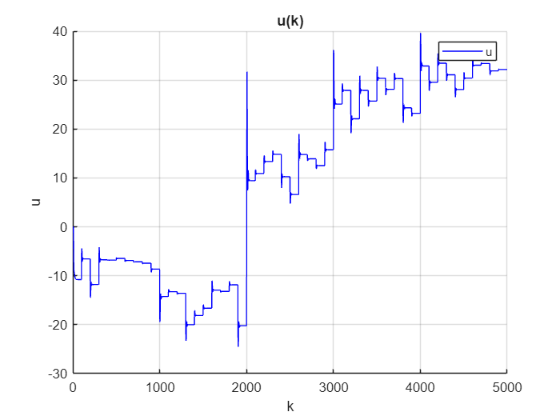
\includegraphics[width=0.8\textwidth]{pictures/dmc_analitic_u}}
\caption{Algorytm analityczny DMC z pomiarem zakłóceń.}
\end{figure}

\newpage

\begin{figure}[h!]
\centering
\subfloat{
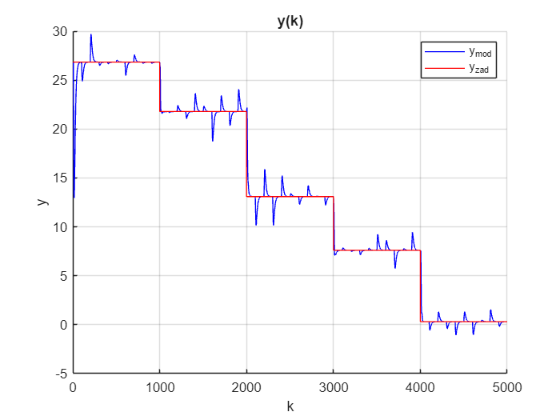
\includegraphics[width=0.8\textwidth]{pictures/dmc_numeric_y_z}}
\hfill
\subfloat{
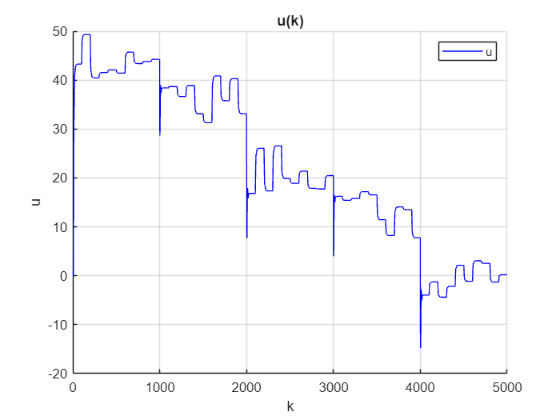
\includegraphics[width=0.8\textwidth]{pictures/dmc_numeric_u_z}}
\caption{Algorytm numeryczny DMC bez pomiaru zakłóceń.}
\end{figure}

\newpage

\begin{figure}[h!]
\centering
\subfloat{
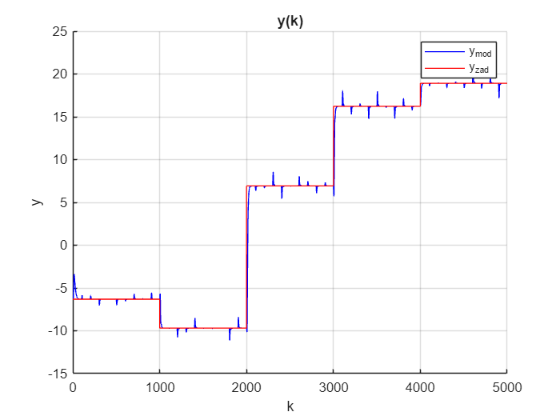
\includegraphics[width=0.8\textwidth]{pictures/dmc_numeric_y}}
\hfill
\subfloat{
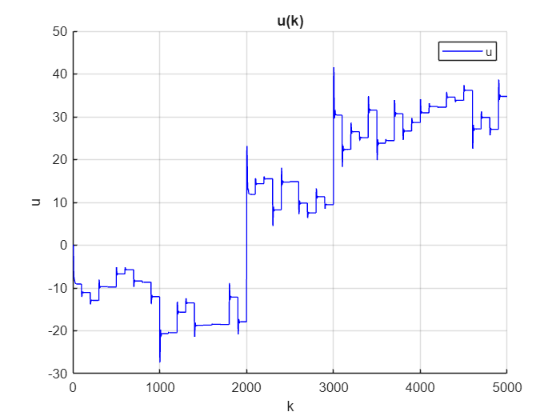
\includegraphics[width=0.8\textwidth]{pictures/dmc_numeric_u}}
\caption{Algorytm numeryczny DMC z pomiarem zakłóceń.}
\end{figure}

Na podstawie przedstawionych przebiegów można wysnuć następujące wnioski:

\begin{itemize}
\item[•] algorytm numeryczny potrafi uwzględnić ograniczenia sygnału sterującego, dzięki temu nie zaobserwowano bardzo dużych przyrostów sterowania
\item[•] pomiar zakłóceń zarówno w wersji analitycznej, jak i numerycznej przynosi bardzo duże korzyści w jakości sterownia 
\end{itemize}
\chapter{Podsumowanie}
W trakcie wykonywania projektu oraz identyfikując dany obiekt regulacji automatycznej nasunęło się kilka wniosków, które postarano się opisać poniżej.

Modele Hammersteina składają się z nieliniowego bloku wejściowego, który jest połączony szeregowo z liniowym dynamicznym blokiem. Nieliniowość jest zazwyczaj statyczna i jest aplikowana do sygnału wejściowego przed jego przetworzeniem przez liniowy system dynamiczny. Ten rodzaj modelu jest używany do opisu systemów, gdzie nieliniowość występuje na wejściu, a reszta systemu zachowuje się liniowo. Modele Hammersteina są użyteczne w identyfikacji systemów i projektowaniu regulatorów.

Modele Wienera, odwrotnie do modeli Hammersteina, mają liniowy dynamiczny blok na wejściu, który jest połączony szeregowo z nieliniowym blokiem wyjściowym. Liniowy blok dynamiczny przetwarza sygnał wejściowy, który następnie przechodzi przez nieliniowy blok. Modele te są stosowane, gdy nieliniowość występuje na wyjściu systemu, po przetworzeniu przez liniowy system dynamiczny. Modele Wienera są przydatne w analizie systemów z nieliniowymi elementami wyjściowymi.

Stosowanie modeli Hammersteina i Wienera w obiektach regulacji automatycznej jest ważne, ponieważ pozwalają one na dokładniejsze modelowanie rzeczywistych systemów, które często zawierają zarówno elementy liniowe, jak i nieliniowe. Dzięki nim można lepiej zrozumieć zachowanie takich systemów i opracować bardziej precyzyjne i skuteczne strategie regulacji. To z kolei prowadzi do poprawy wydajności, stabilności i niezawodności systemów automatyki. Integracja tych modeli w procesie projektowania systemów automatyki umożliwia także lepsze przewidywanie i kompensowanie nieliniowych efektów w działaniu systemów.

Jak można było zauważyć na zaprezentowanych wykresach, zaimplementowanie nieliniowej statyki, którą poprzedzała, bądź występowała po niej, liniowa dynamika diametralnie poprawiała jakość opisu obiektu. W każdym z rozpatrywanych przypadków udało się osiągnąć założone kryterium jakości, którym był błąd średnio kwadratowy, nie większy niż $\num{0.1}$. 


\listoffigures
%\listoftables
\end{document}